\documentclass[../ECE459FinalProjectReport.tex]{subfiles}

\begin{document}
\chapter{Methodology}
The project simulates the AM and FM communication systems respectively which applies Python 3. The work is done using Jupyter Notebook. Packages imported include \verb|numpy| for numerical computation, \verb|scipy| for signal analysis, and \verb|matplotlib| for plotting.

\section{AM Simulation}
\subsection{Envelope Modulation}

\subsection{Envelope Detection}

\subsection{SNR Calculation and Measurement}

\section{FM Simulation}
\subsection{Narrow-Band FM Modulation}

\subsection{Narrow-Band FM Demodulation}

\subsection{SNR Calculation and Measurement}

\section{Filter Design}
\subsection{Ideal Filters}
% 讲LPF和BPF的TF,然后引出为什么ideal filter无法实现,再引出butterworth

\subsection{Butterworth Filter}

Both AM and FM communication systems require filters. Yet in real life, ideal filters are not implementable. However, the Butterworth Filter can behave closely to the ideal filter. According to \cite{storrButterworthFilterDesign2013,kudekiAnalogSignalsSystems2009}, a Butterworth Low Pass Filter has a maximum flat frequency response within its passband and rolls off quickly at the cut-off frequency.

The transfer function of a Butterworth Low Pass Filter is expressed as
\begin{equation}
    \left| H\left( \omega \right) \right|^2=\frac{1}{1+\left( \frac{\omega}{\omega _c} \right) ^{2n}}
\end{equation}
where $n$ is the order of the filter and $\omega_c$ is the cut-off frequency. The higher the order $n$, the closer the Butterworth Filter behaves like an ideal filter.


\begin{figure}[b]
    \centering
    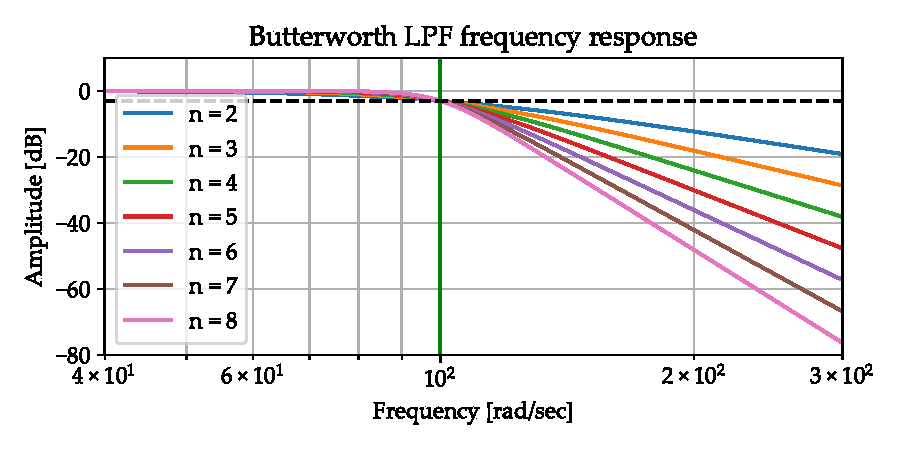
\includegraphics[scale=0.7]{plots/butterworth-lpf.pdf}
    \caption{The frequency response of a Butterworth LPF with cut-off frequency $\omega_c = \SI{100}{\radian\per\s}$. The black dash line shows the \SI{-3}{\dB} amplitude.}
    \label{fig:butter-lpf}
\end{figure}

\begin{figure}[b]
    \centering
    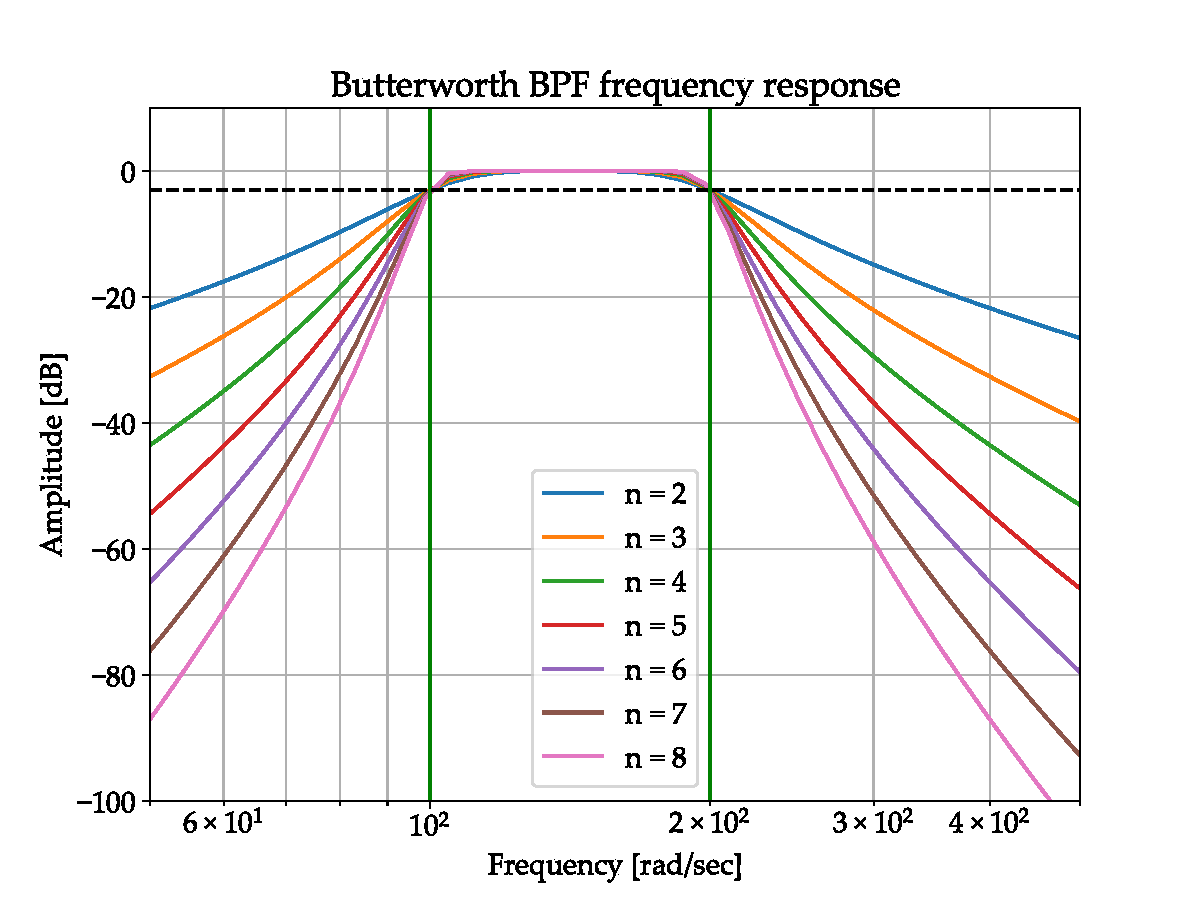
\includegraphics[scale=0.7]{plots/butterworth-bpf.pdf}
    \caption{The frequency response of a Butterworth BPF with cut-off frequency $\omega_c = \SI{100}{\radian\per\s}$. The black dash line shows the \SI{-3}{\dB} amplitude.}
    \label{fig:butter-bpf}
\end{figure}


\section{Additive White Gaussian Noise}
% Definition, principles, and how to generate in Python

\end{document}